\section{PKI and WoT}

Before describing the two types of security systems, we need to understand the basic 
Cryptography Security goals, or CIA and the importance of public and private keys 
for cryptographic security\cite{b31}.
\begin{enumerate}[]
    \item \textbf{Confidentiality}: only entitled entities may be able to read the data.
    \item \textbf{Integrity}: tampering with a message will be detected.
    \item \textbf{Authenticity}: the communicating parties can be identified/verified.
    \end{enumerate}
\\
These are our core security goals.
\begin{figure}[H] %H为当前位置,!htb为忽略美学标准,htbp为浮动图形
    \centering %图片居中
    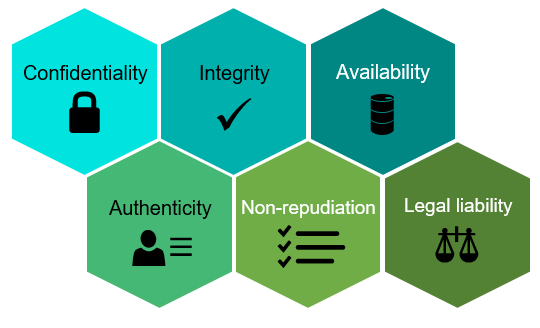
\includegraphics[width=0.3\textwidth]{figures/cia.png} %插入图片,[]中设置图片大小,{}中是图片文件名
    \caption{the basic cryptography security goals} %最终文档中希望显示的图片标题
    \label{Fig.2: the basic Cryptography Security goals} %用于文内引用的标签
\end{figure}
In addition, we might also have other goals:
\begin{enumerate}[]
    \item \textbf{Non-repudiation}: a communication partner cannot deny a message originated from her.
    \item \textbf{Forward secrecy}: compromise at this point in time does not lead to compromise of past connections.
    \item \textbf{Availability}: systems and data are available to individuals when they need it under any circumstances, including power outages or natural disasters.
    \end{enumerate}
\\
Attackers may listen in on messages in transit as well as manipulate them at will. An example
for a passive attack is eavesdropping: Alice sends Bob a message. Eve is listening on the line.
Thus, she can also see the message. Now she knows what Alice said. She eavesdropped on
Alice and Bob.


\subsection{PKI - Public Key Infrastructure}
One possible way of formalizing confidentiality is the Choice Plaintext Attack (CPA): 
an algorithm can provide confidentiality if a theoretical adversary is allowed to require 
the encryption of any plaintext and still not be able to obtain any information from the 
ciphertext\cite{b38}. Cryptography uses such models to analyze the security properties of a structure. 
CPA security algorithms provide encryption\cite{b31}.
\\
However, guarding against CPA does not help us defend against active attackers. Active 
attackers can manipulate messages. To prevent manipulation and forgery, we add authenticators 
to messages, such as message authentication tags\cite{b38}. The algorithm provides authenticity if 
the adversary is allowed to obtain the authentication tag of any message of its choice, 
but still cannot compute a valid authentication tag for the new message. This is called 
security under a chosen-ciphertext attack, which provides message authentication.
These security properties require certain assumptions that we will not discuss in detail 
here, such as the polynomial running time of the adversary and access to random bits.

\subsubsection{private-key cryptography}\cite{b38}
In the private key (symmetric) encryption setup, we assume that the communication partners 
have securely exchanged shared keys, one of which is typically 128 bits in length.
\\
A different key must be used for each direction of communication and for each purpose 
(e.g., encryption and authentication).
\\
We use encryption to provide confidentiality for the message m
\\
$k \ = \ Gen(1^n)$
\\
$c \ = \ Enc_k(m)$
\\
$m \ := \ Dec_k(c)$
\\
Enc can be realized with functions such as AES-CTR or ChaCha20.
We use a message authentication code, e.g., HMAC-SHA2, to provide authenticity and 
integrity by generating a message authentication tag t for a message m:
\\
$k \ = \ Gen(1^n)$
\\
$t \ = \ Mac_k(m)$
\\
$b \ := \ Vrfy_k(m, t)$
\\
where b can take both valid and invalid forms.
In order to obtain a reasonably expected level of security, we always want the message 
to have both: authenticated encryption.

\subsubsection{public-key cryptography}\cite{b38}
\\
We use public key (asymmetric) cryptography for three main purposes: confidentiality, 
authentication, and key exchange. In a public key scheme, each party has a key pair 
consisting of a private key sk and a corresponding public key pk.
\begin{figure}[H] %H为当前位置,!htb为忽略美学标准,htbp为浮动图形
    \centering %图片居中
    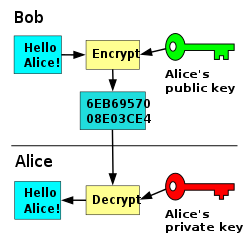
\includegraphics[width=0.3\textwidth]{figures/public_key.png} %插入图片,[]中设置图片大小,{}中是图片文件名
    \caption{public-key cryptography} %最终文档中希望显示的图片标题
    \label{Fig.2: public-key cryptography} %用于文内引用的标签
\end{figure}
Encryption is performed using the receiver's public key and decryption is performed 
by the receiver using his private key and vice versa.
\\
$(pk, sk) \ = \ Gen(1^n)$
\\
$c \ = \ Enc_{pk}(m)$
\\
$m \ := \ Dec_{sk}(c)$
\\
Encryption algorithms can be based on RSA or ECDH issues, such as RSA-OAEP.
\\
Signatures are created using a private key and verified using the corresponding public key. 
They provide not only authenticity but also non-repudiation. Examples of signature algorithms 
are Ed25519 and RSA-PSS.
\\
$(pk, sk) \ = \ Gen(1^n)$
\\
$s \ = \ Sign_{sk}(m)$
\\
$b \ := \ Vrfy_{pk}(m, s)$
\\
Because public-key encryption is typically slower than secret-key encryption, it is often 
used in handshakes to utilize key distribution properties and generate shared secret keys, 
which are then used to protect bulk traffic.
\\
Using cryptography correctly is only a small part of creating a secure system. Many things 
can still go wrong, such as side-channel attacks, buffer overflows, or other errors.
\\
It's easy to try to use cryptography to solve security problems, but the problems are often 
more complex and our assumptions ultimately prove invalid. Consider the following common problems:

\begin{enumerate}[]
    \item[*] side channels
    \item[*] inadequate threat model
    \item[*] replay attacks
    \item[*] traffic analysis
    \item[*] baseboard management controllers
    \item[*] correct behaviour is difficult for users
    \end{enumerate}

\subsubsection{Signatures and Certificates}\cite{b38}
Digital signatures are the cyberspace version of handwritten signatures. Both digital and 
handwritten signatures are sent with the original data to provide authentication.
\begin{figure}[H] %H为当前位置,!htb为忽略美学标准,htbp为浮动图形
    \centering %图片居中
    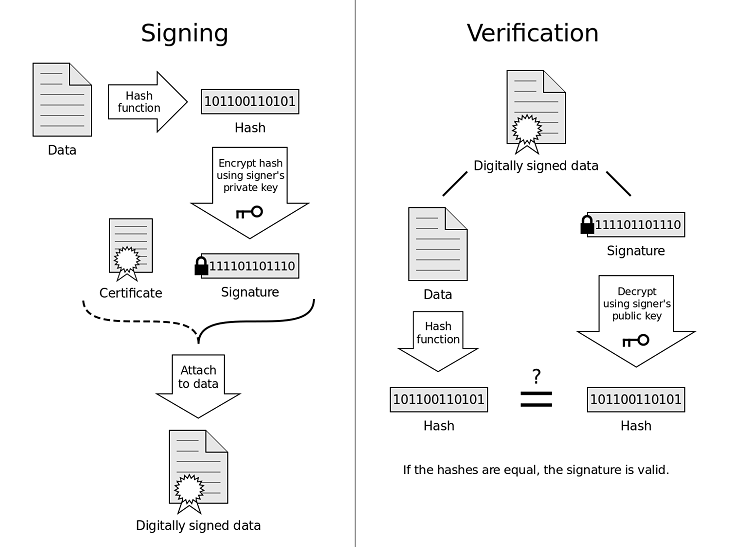
\includegraphics[width=0.5\textwidth]{figures/signature.png} %插入图片,[]中设置图片大小,{}中是图片文件名
    \caption{signatures and certificates} %最终文档中希望显示的图片标题
    \label{Fig.2: Signatures and Certificates} %用于文内引用的标签
\end{figure}
In addition, both are inseparable from the original data. In fact, the signature is not 
inextricably linked. They can be removed by simply cutting out the appropriate portion of 
the original document. However, this destroys the validity of the document.
\\
Handwritten signatures are usually placed at the bottom of the same sheet of paper that 
contains the data that the signer (Alice) wants to confirm in writing. Imagine that the 
situation would be different.
\\
Imagine a contract and a signature written on two different pieces of paper. This could 
be abused. For example, having the piece of paper with the signature, the recipient of the contract
signature (Bob) can reuse it to sign everything he wants (without asking Alice's permission).
\\
Let's return to digital signatures. Similar to the handwritten version, the digital 
signature sits after the original data. But instead of paper, we have packets and streams 
of data.
\\
In the context of TLS, however, we don't have contracts, only certificates, "which are 
data structures that bind public key values to subjects." (RFC 5280) More specifically, 
we have X.509 certificates here. The previous quote sounds rather complex and abstract, 
but it's actually not that difficult. The certificate for web server Bob (the subject) 
proves that Bob is the owner of the public key $K_{pubBOB}$ given in the certificate. 
Knowing this, Alice can determine one thing:
\\
Using $K_{pubBOB}$ to encrypt the data, only one person can decrypt and read the data.
\\
Guess who... The owner of the corresponding private key $K_{privBOB}$, of course. 
Assuming this key is stored securely, the only person who knows $K_{privBOB}$ is Bob. 
Therefore, by binding Bob to $K_{pubBOB}$, Alice can securely send data to Bob. It is 
important to understand these correlations.
\\
One question remains open. How does the binding happen? Now we can close the loop. 
Binding occurs through signatures. The signature is given by a trusted third party, 
thus confirming, "Yes, I know and guarantee that Bob and $K_{pubBOB}$ do belong together." 
The identity of that person and the mystery of trust in that context will be revealed 
on the next page, in "Public Key Infrastructure".
\\
But regarding trust in handwritten signatures, have you ever actually verified the 
signature of the person who signed the document you received. Imagine these three scenarios:
\begin{itemize}
    \item[*] Both parties to the contract were present when it was signed. This is similar to the situation where Alice physically walks to Bob's house and obtains Bob's public key.
    \item[*] Since Alice already has the document with Bob's signature, she can verify Bob's signature by comparing the two signatures on the two documents. This is equivalent to the case where Alice already knows Bob's public key.
    \item[*] Alice just believes that the signature is indeed signed by Bob. Otherwise someone is breaking the law. This is analogous to the case where Alice trusts a trusted third party who signed the certificate.
\end{itemize}

\subsubsection{Transport Layer Security}\cite{b38}

\begin{figure}[H] %H为当前位置,!htb为忽略美学标准,htbp为浮动图形
    \centering %图片居中
    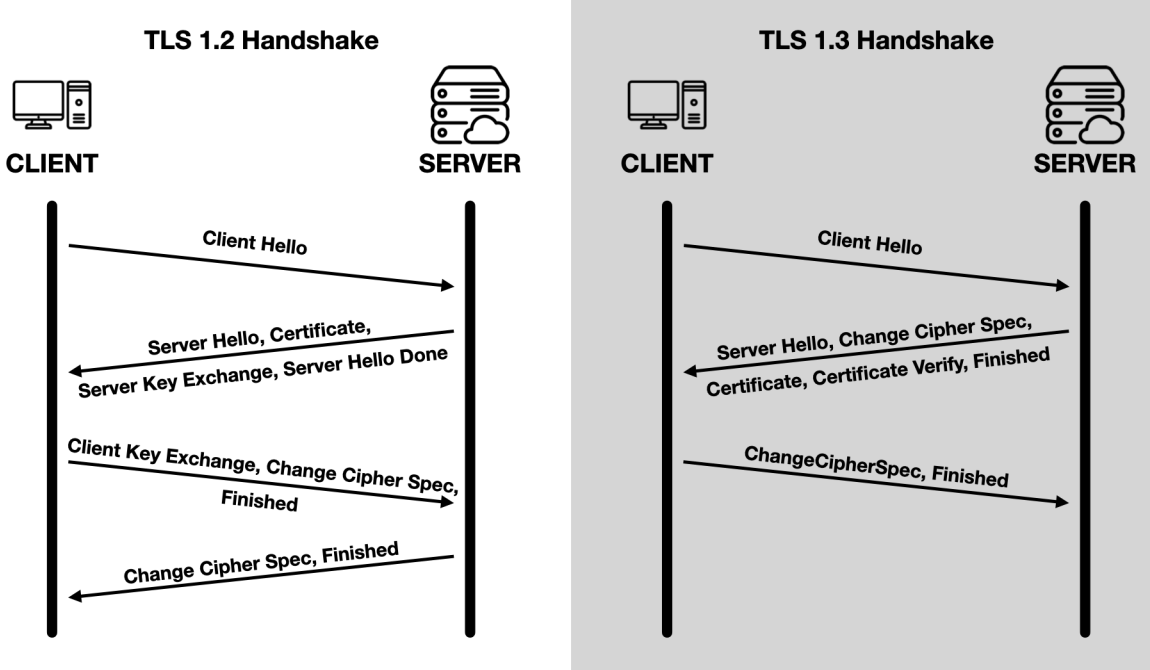
\includegraphics[width=0.5\textwidth]{figures/TLS.png} %插入图片,[]中设置图片大小,{}中是图片文件名
    \caption{TLS 1.2 and TLS 1.3 handshake} %最终文档中希望显示的图片标题
    \label{Fig.2: TLS 1.2 and TLS 1.3 handshake} %用于文内引用的标签
\end{figure}

TLS stands for Transport Layer Security, a protocol used to protect Layer 4 traffic. 
While researching more about it, you may stumble upon the term SSL (Secure Sockets Layer), 
which is the predecessor to TLS.
\\
The Internet Engineering Task Force (IETF) released TLS 1.3 in August 2018. The version it 
replaces, TLS 1.2, was standardized a decade ago in 2008, but it is still widely deployed 
and is only slowly being replaced by its successor.
\\
The diagram above \ref{Fig.2: TLS 1.2 and TLS 1.3 handshake} briefly summarizes the 
TLS 1.2 and TLS 1.3 handshakes. You can see a 
representation of each of the 4 main segments of TLS 1.2 and the 3 segments of TLS 1.3.

\subsubsection{Diffie-Hellman-Key-Exchange}\cite{b38}
A fundamental problem when using symmetric keys is how to exchange them without anyone 
knowing or generating them, so that ultimately the two parties involved share the same 
key. One method of communicating without a secure channel is Diffie-Hellman-Key-Exchange.
\\
During the handshake, both parties agree on the parameters of the key derivation in the 
exchange message. Knowing them does not help an attacker understand the key. The basic 
principle of key derivation between Alice and Bob is the following scheme:

\begin{enumerate}[]
    \item[*] Alice and Bob agree on two parameters $g$ and $p$ for the key export. This can be done by Alice simply choosing them and sending them to Bob.
    \item[*] Both then generate a random number. This number is known only to them and will not be sent anywhere. Using this random number, Alice calculates $A \ = \ g^a \ mod \ p$ and Bob calculates $B \ = \ g^b \ mod \ p$. A and B are then sent to their respective other partners.
    \item[*] They can now both generate the shared key K by computing $K \ = \ B^a \ mod \ p$ and $K \ = \ A^b \ mod \ p$.
    \end{enumerate}
\\
Alice and Bob now share the same key K. The important thing here is that it is not possible 
to derive K by knowing g, p, A, and B. For this, the attacker needs to keep the random numbers 
a and b secret.

\subsubsection{Certificate Authority}\cite{b38}
Let's consider the previous question. But whose key is it? It is the public key of an 
organization called a Certificate Authority (CA). The CA issues the certificate and 
also signs it using its private key. The signing is actually performed by a 
Registration Authority (RA). In many cases, the CA also assumes the role of the RA. 
For the sake of clarity, we will consider here a CA that also signs the certificates 
it issues.
\\
We can only trust the server certificate if we can rely on the CA. Thus, we are 
simply transferring the trust issue to another entity. However, in PKI, CAs are 
trusted third parties, which means that we have no choice but to trust them or to 
obtain the server's public key on a different secure channel. We don't actually have 
to trust this particular CA. Each CA itself has a certificate, similar to the server's 
certificate. Our CA's certificate is signed by another CA's private key. Once again, 
we are transferring trust. What we have here is a chain of trust, the last link of which 
is the root CA. Since there is no CA above the root CA, there is no CA that can sign 
the root CA's certificate. It is "self-signed". In short, if you trust the root CA and 
find a gapless chain to the CA that signed the server's certificate, then you trust it. 
Usually, browsers provide a list of pre-installed trusted CAs.
\\
In Figure \ref{Fig.2: PKI_Chain_of_Trust}, you can see a graphical representation of 
such a chain of trust. A client requests a service from a server.
\\
Since it is a TLS-protected session, the client asks the server to prove its identity 
with a certificate. It is signed by a $CA_n$. The client has never heard of $CA_n$ and obtains 
a certificate from $CA_n$. It is signed by $CA_{n-1}$. Since the client only knows the root CA, 
it must obtain all certificates until it retrieves one signed by the root CA.

\begin{figure}[H] %H为当前位置,!htb为忽略美学标准,htbp为浮动图形
    \centering %图片居中
    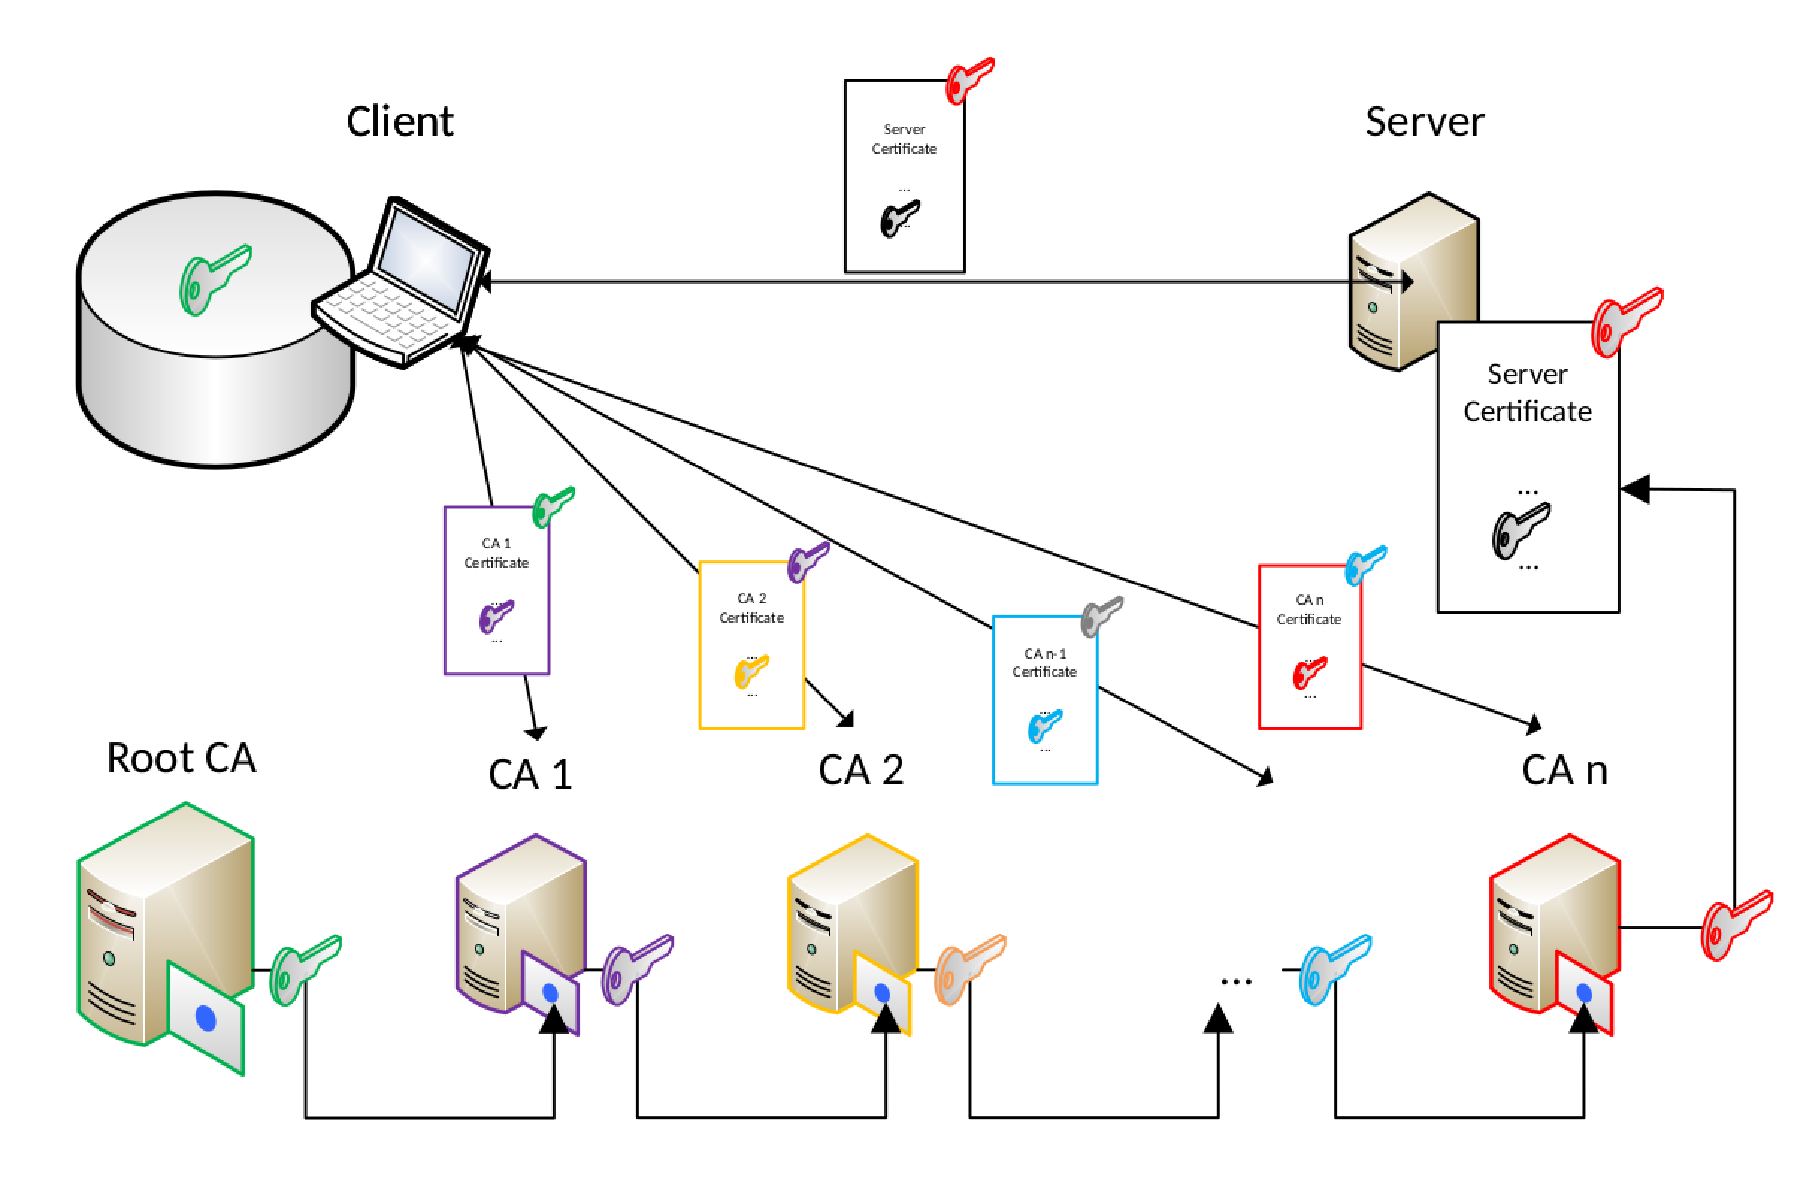
\includegraphics[width=0.5\textwidth]{figures/PKI_Chain_of_Trust.png} %插入图片,[]中设置图片大小,{}中是图片文件名
    \caption{PKI - Chain of Trust} %最终文档中希望显示的图片标题
    \label{Fig.2: PKI_Chain_of_Trust} %用于文内引用的标签
    \end{figure}

\subsubsection{Certification Request}\cite{b38}
Let's consider a server. Before it can prove its identity with a signed certificate, it must 
retrieve one. The certificate binds the identity inextricably to the public key. In addition 
to its identity (e.g., company name) and its proprietary name (domain name, e.g., 
"www.example.com"), the server needs the public key to be used for the certification request 
(CR or certificate signing request CSR). The key pair is generated locally by the server 
and the corresponding private key is kept secret. After all the information has been 
collected, the data is packaged into the authentication request, e.g. in PKCS#10 format. 
To prove that it knows the corresponding private key, the server must sign the CSR. Upon 
receipt of the request, the CA must validate the CSR. This can be done in a number of ways, 
such as forcing the requester to present a passport (although this is less stringent in 
most cases). Once the CSR is verified, the CA issues a signing certificate (e.g., an X.509 
certificate).


\subsection{WoT - Web of Trust}
Web of Trust (WoT)\cite{b7} is a concept in cryptography that can be used to authenticate the 
identity of the holder of a public key, as applied in PGP, GnuPG, or other OpenPGP-compatible 
systems\cite{b8, b9, b10}. Trust networks use the concept of decentralization, unlike public key 
infrastructures that rely on digital certificate certification authorities. In a 
computer network, there can be many independent trust networks at the same time, and 
any user can be a part of one of these networks, or a link between different networks\cite{b11}.
\\
In PKI, all trust stems from trust in the CA organization, but CA organizations can make 
mistakes. Even those CA organizations that have not made any errors so far, there is 
no guarantee that they will not make errors in the future. In contrast to PKI, where 
there is unconditional trust in CAs, another type of PKI is called a "network of trust", 
where there are no CAs, but rather a network built on one-to-one trust\cite{b7}.

\begin{figure}[H] %H为当前位置,!htb为忽略美学标准,htbp为浮动图形
    \centering %图片居中
    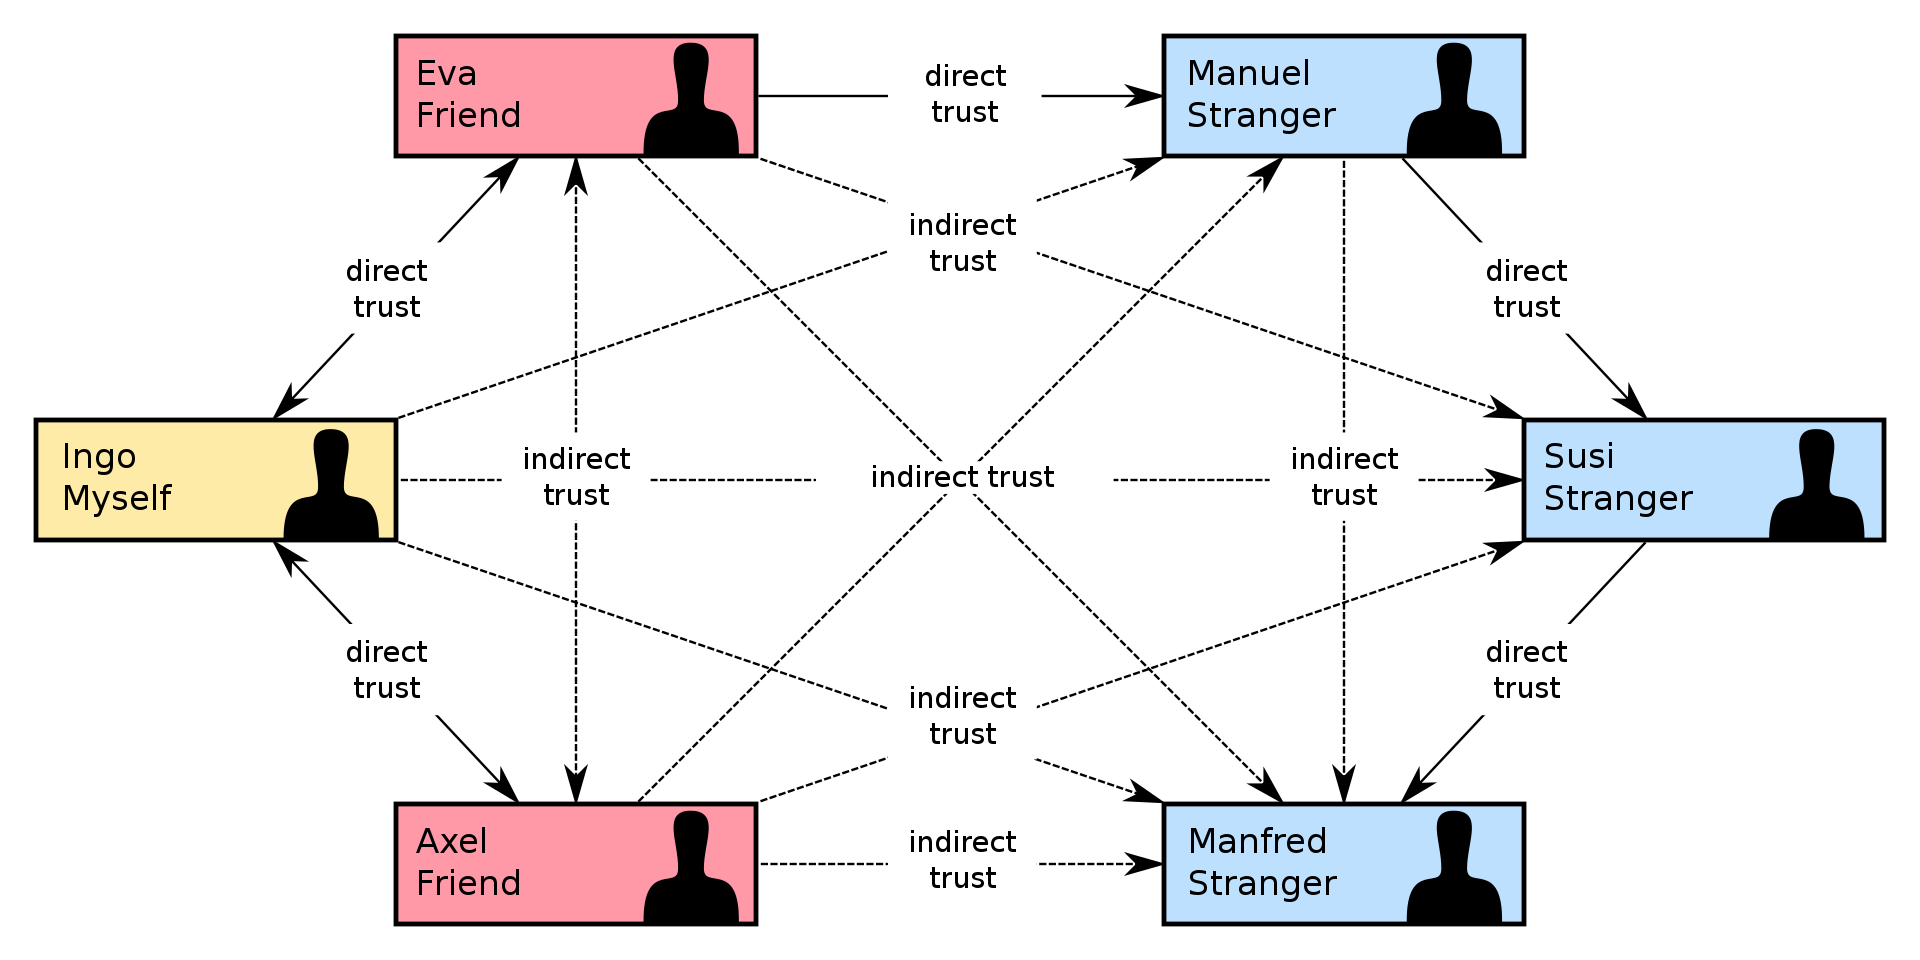
\includegraphics[width=0.5\textwidth]{figures/decentralized_trust_model.png} %插入图片,[]中设置图片大小,{}中是图片文件名
    \caption{The decentralized trust model} %最终文档中希望显示的图片标题
    \label{Fig.2: decentralized_trust_model} %用于文内引用的标签
    \end{figure}
\\
The concept of trust networks was first introduced by PGP author Philip Zimmermann in 
the PGP 2.0 manual\cite{b7}.
\\
Over time, you will gradually collect many other people's keys, some of whom you may 
be willing to sign up to trust (treating them as trusted introducers). Other people 
will also sign up for some other people's keys that they themselves trust (choosing 
their own trusted introducers).
\\
Each person gradually accumulates a number of keys that have been signed and trusted 
by others, and then signs and distributes them himself. Then one can expect that the 
next person to get the key will always have one or two people on the signing list that 
he or she trusts. This eventually creates a distributed, cheat-proof trust network of 
all public keys.
\\
This is the idea of trust in a network of trust. When any user uses someone else's 
public key, he becomes a referrer of that public key. When such a procedure is 
continued, a network of trust is formed where all public keys are decentralized 
and fault-tolerant.

\begin{figure}[H] %H为当前位置,!htb为忽略美学标准,htbp为浮动图形
    \centering %图片居中
    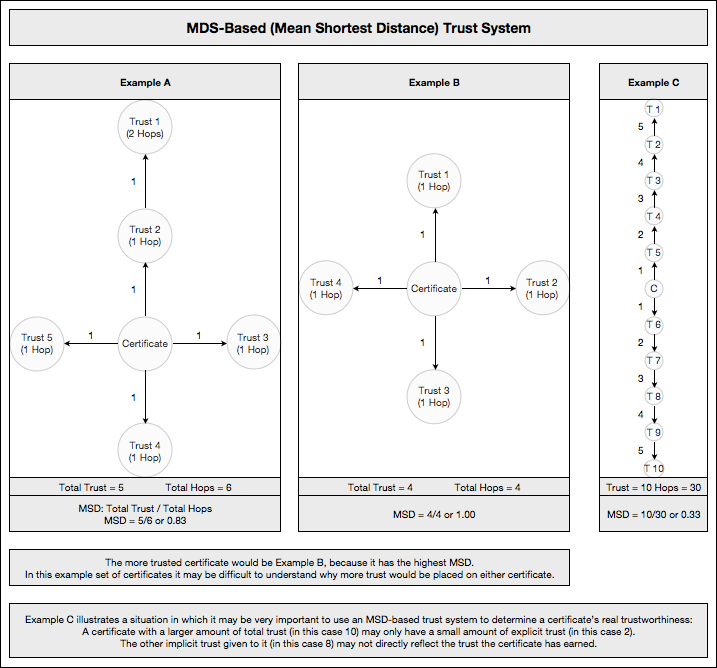
\includegraphics[width=0.5\textwidth]{figures/trustSystem.png} %插入图片,[]中设置图片大小,{}中是图片文件名
    \caption{MDS-Based (Mean Shortest Distance) Trust System} %最终文档中希望显示的图片标题
    \label{Fig.2: MDS-Based (Mean Shortest Distance) Trust System} %用于文内引用的标签
    \end{figure}

\\
In a trust network, any trust network user can verify the public key credentials of other 
trust network users. However, such credentials are only trusted if the third party also 
considers the verifier to be a trusted referrer. (That is, if you want to trust a key that 
I think is valid, you have to recognize me as a trusted referrer. Otherwise my validation 
for another key is meaningless to you.)
\\
What is stored in each user's public keystore contains the following information:
\\
Whether a key is considered valid by the user.
\\
The degree to which the user trusts that key, which relates to the key owner's 
ability to be a verifier of other keys.
\\
You point out the counts on my comment based on my copy of the key.
\\
It's really a reputation system: some people have a good reputation for being 
trusted, and people thus trust that their verification of other keys is valid.

\subsubsection{Direct Trust}
Direct trust is the simplest model of trust. In this model, the user trusts a 
key to be valid because they know where it came from\cite{b27}. All cryptosystems use this 
form of trust to some extent. For example, in web browsers, CA agency root 
certificates are trusted directly because they are built into the operating system 
and browser\cite{b28}.

\begin{figure}[H] %H为当前位置,!htb为忽略美学标准,htbp为浮动图形
    \centering %图片居中
    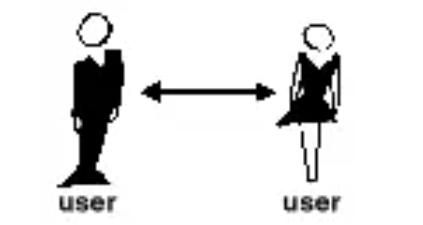
\includegraphics[width=0.2\textwidth]{figures/directTrust.png} %插入图片,[]中设置图片大小,{}中是图片文件名
    \caption{Direct Trust} %最终文档中希望显示的图片标题
    \label{Fig.3: Direct Trust} %用于文内引用的标签
    \end{figure}


\subsubsection{Trust Tree}
In the chain of trust, there will be a number of trusts extended from the "root 
certificate". These certificates may vouch for themselves, or vouch for certificates 
at lower levels. Think of this as a chain of trust\cite{b31}. The authenticity of a downstream 
certificate is proven by the authenticity of the certificate that issued it, until 
it is directly trusted by the root certificate. From an individual perspective, this 
is a chain of trust, while from a holistic perspective, it is actually a tree of trust\cite{b28}.

\begin{figure}[H] %H为当前位置,!htb为忽略美学标准,htbp为浮动图形
    \centering %图片居中
    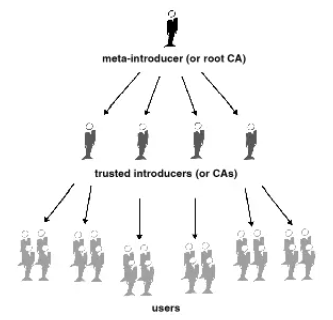
\includegraphics[width=0.4\textwidth]{figures/trustTree.png} %插入图片,[]中设置图片大小,{}中是图片文件名
    \caption{Trust Tree} %最终文档中希望显示的图片标题
    \label{Fig.4: Trust Tree} %用于文内引用的标签
    \end{figure}


\subsubsection{Trust Network}
\begin{figure}[H] %H为当前位置,!htb为忽略美学标准,htbp为浮动图形
    \centering %图片居中
    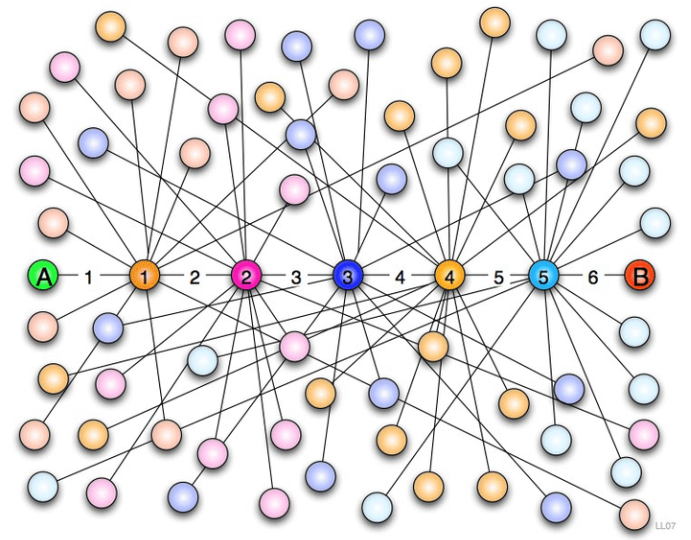
\includegraphics[width=0.4\textwidth]{figures/trustNet.png} %插入图片,[]中设置图片大小,{}中是图片文件名
    \caption{Trust Network} %最终文档中希望显示的图片标题
    \label{Fig.5: Trust Network} %用于文内引用的标签
    \end{figure}
A trust network differs from the above two models in that a trust network can be 
thought of as a network of several direct trusts connected together. In a trust 
network\cite{b27}, you believe that a key is real because someone you trust believes it to 
be real. This person is called the introducer\cite{b28}.
\\
You may have heard of the Six Degrees of Separation theory\cite{b37}: that any two people 
in the world who don't know each other need up to six intermediaries to be able 
to make a connection\cite{b29}.


\subsubsection{PGP}
The Privilege and Secrecy Protocol (PGP) is one such security protocol based on 
a network of trust\cite{b11}.The biggest difference between PGP and other security protocols 
is the way he verifies the certificates - based on a network of trust, instead of PKI 
and root certificates\cite{b12}.
\\
In PGP, there are three levels of trust for a key:

\begin{enumerate}[]
    \item \textbf{Complete Trust}
    \item \textbf{Suspicion}
    \item \textbf{Complete Distrust (or lack of trust)}
    \end{enumerate}
\\
Only a key that is fully trusted by one referrer, or half-trusted by two referrers, 
can be determined to be a valid key.

\begin{figure}[H] %H为当前位置,!htb为忽略美学标准,htbp为浮动图形
    \centering %图片居中
    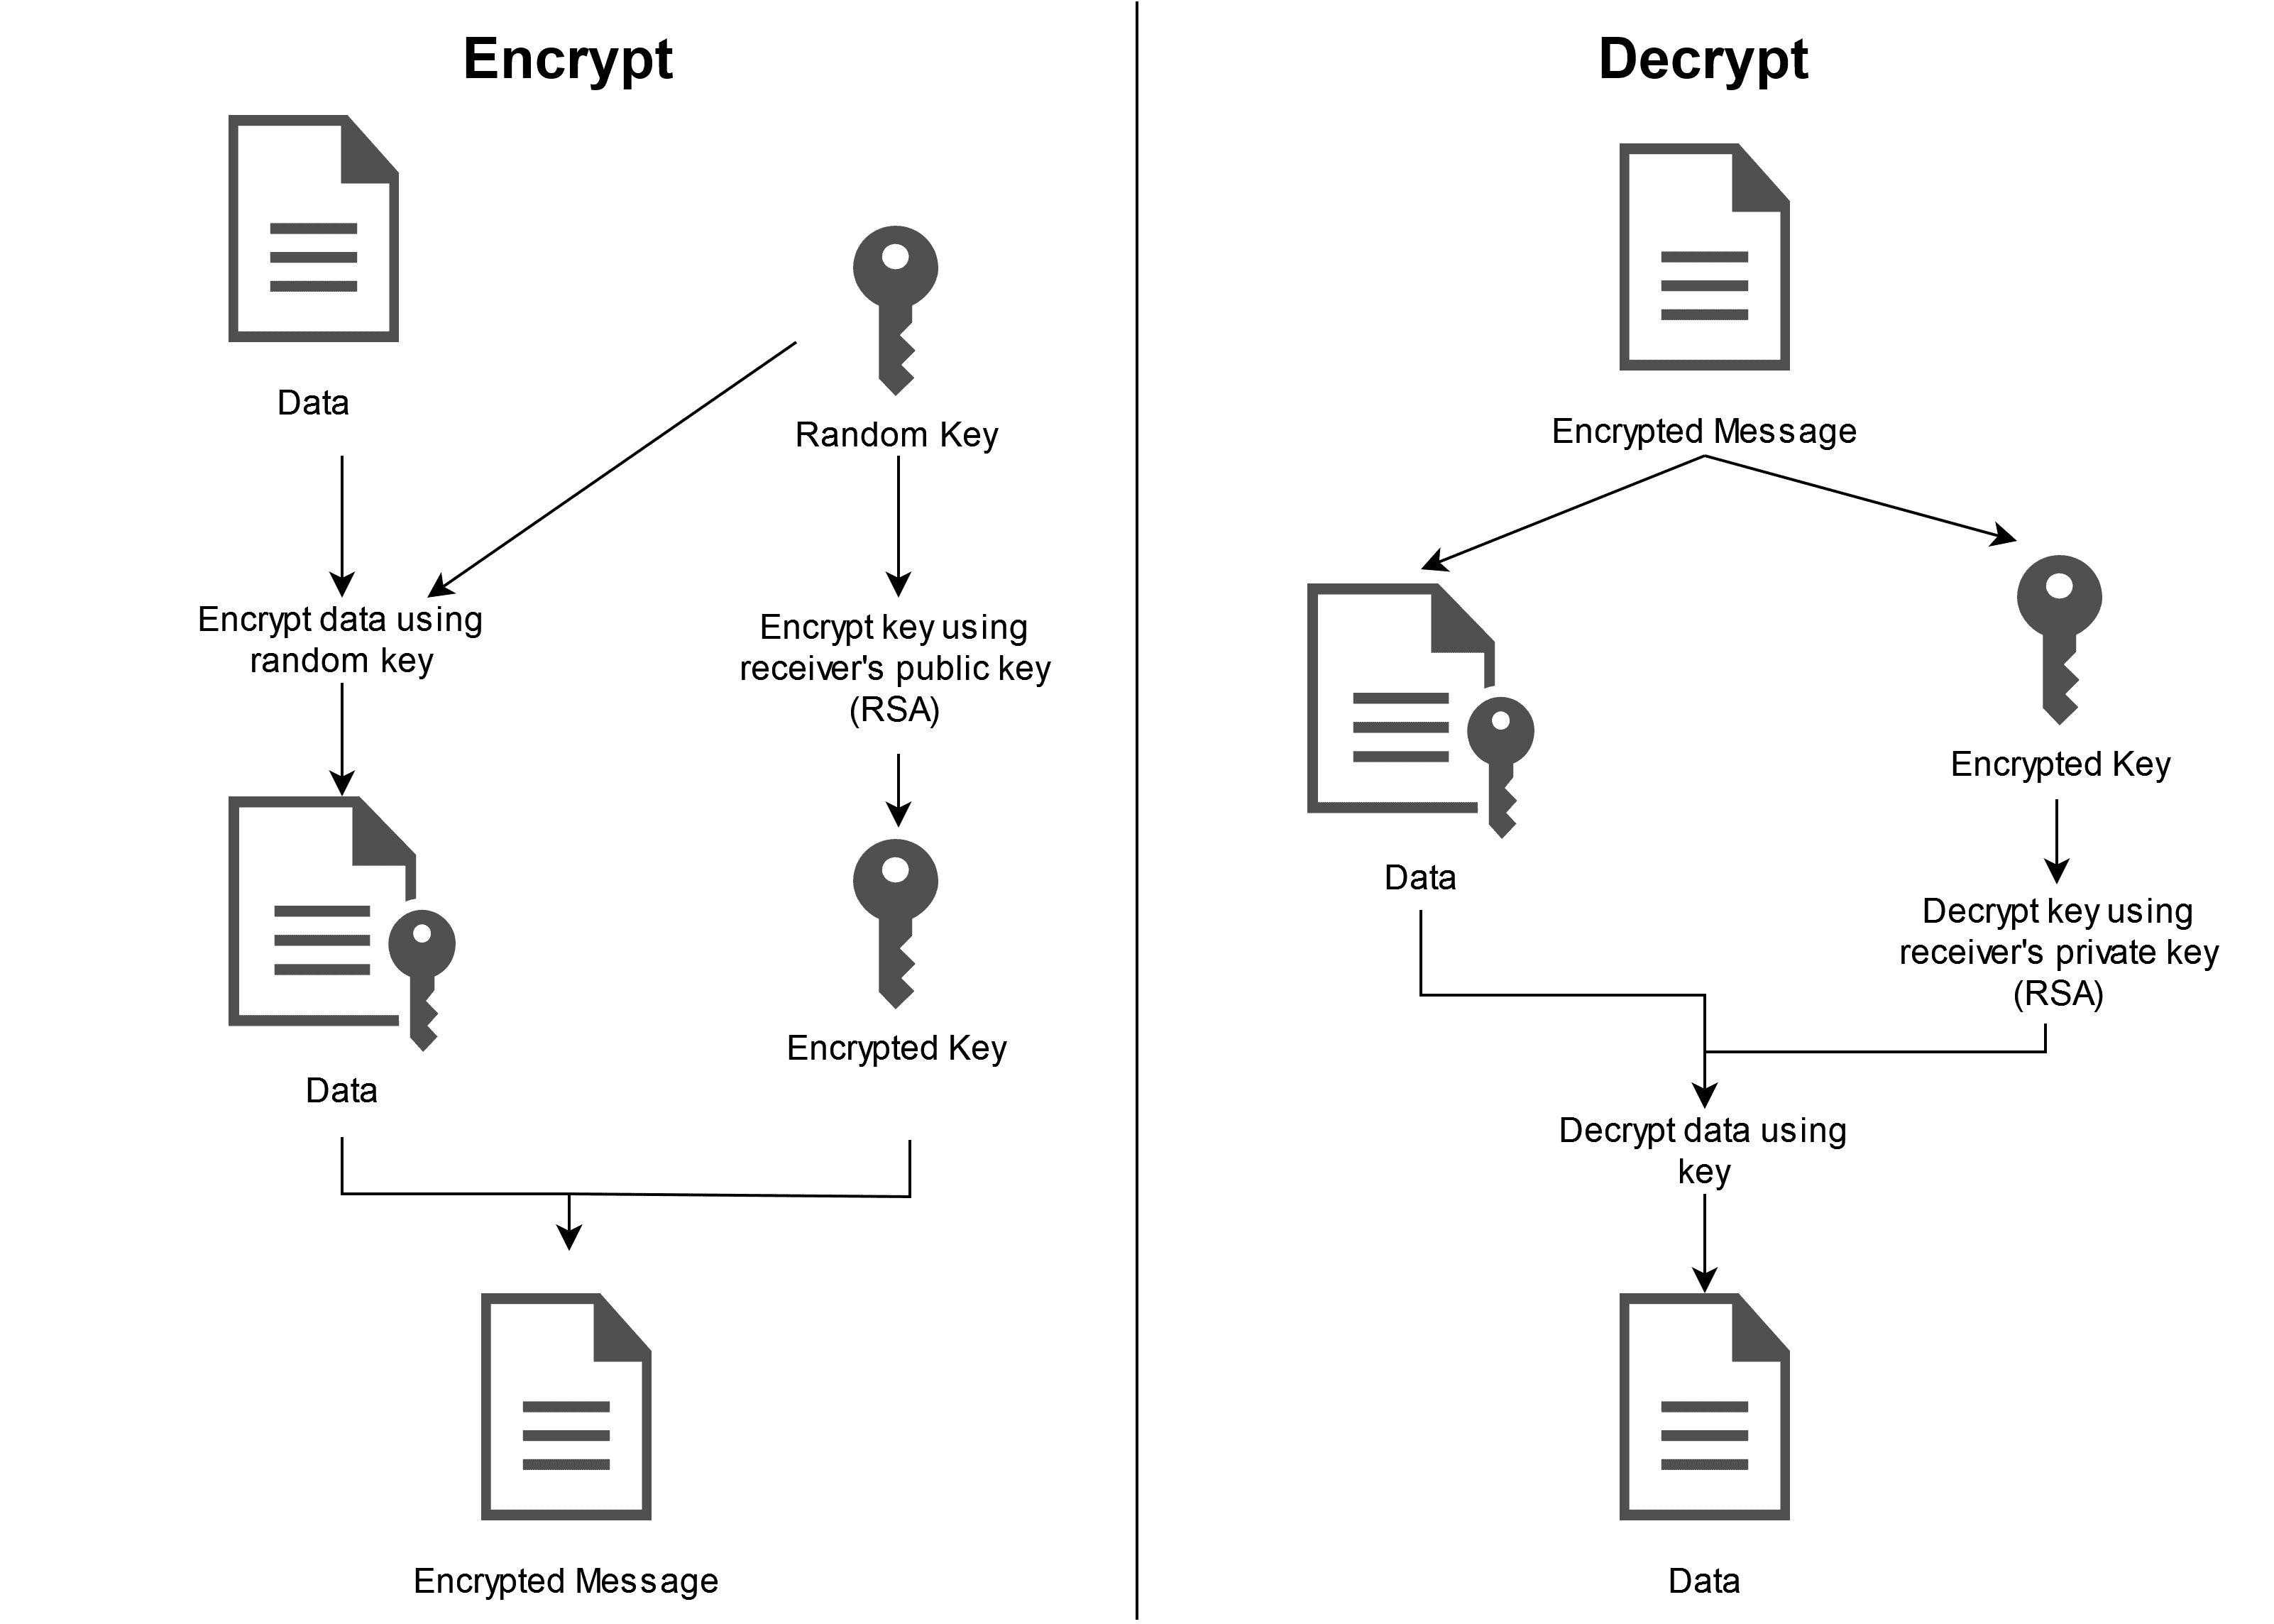
\includegraphics[width=0.5\textwidth]{figures/PGP.png} %插入图片,[]中设置图片大小,{}中是图片文件名
    \caption{PGP} %最终文档中希望显示的图片标题
    \label{Fig.6: PGP} %用于文内引用的标签
    \end{figure}
\\
In PGP, we no longer rely on CA organizations to help us check the authenticity of 
certificates, we only trust our own judgment. The concept of decentralization embedded 
in it will bring us more reliable and secure encrypted communication\cite{b36}.